%!TEX root =../../../course-notes.tex
% ^ leave for LaTeXTools build functionality
\begin{applicationActivities}


\begin{observation}
A vector field \(\langle P,Q\rangle\) corresponds to the slope field of the differential equation \[\frac{dy}{dx}=\frac{Q}{P}.\]
\vfill
Thus, a solution to this ODE describes the path taken by the particle in this fluid flow.

\begin{center}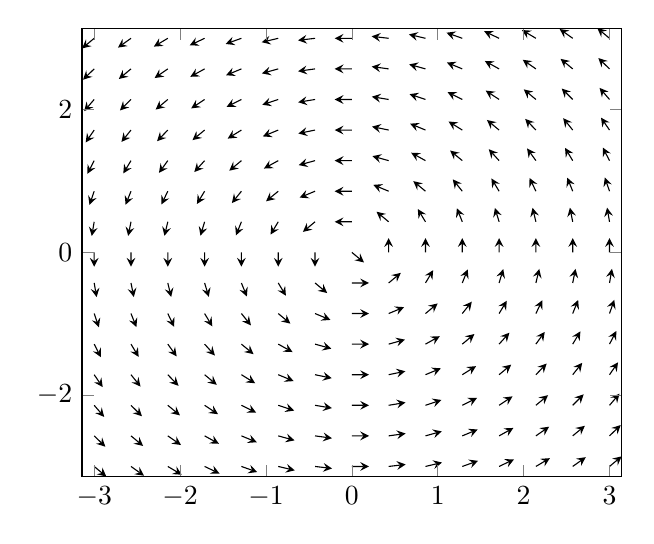
\begin{tikzpicture}
    \begin{axis}[
        domain=-3:3,
        view={0}{90},
        axis background/.style={fill=white},
    ]
        \addplot3[black,
            quiver={
             u={-y/(sqrt(x^2+y^2))},
             v={x/(sqrt(x^2+y^2))},
             scale arrows=0.2,
            },
            -stealth,samples=15]
                {exp(-x) - 1/2*sin(x) - 1/2*cos(x)};
    \end{axis}
\end{tikzpicture}\end{center}


\end{observation}

\begin{activity}{10}
Consider the  ODE \[\frac{dy}{dx} = \frac{-2xy^2-1}{2x^2y}.\]

This can be rewritten as \[ (2xy^2+1) + 2x^2y \frac{dy}{dx} = 0 .\]
\vfill
Now, consider \(\phi(x,y)=x^2y^2+x \).  
\begin{subactivity}
Compute \(\nabla \phi \).
\end{subactivity}
\begin{subactivity}
Differentiate the equation \(\phi(x,y)=c\) with respect to \(x\).
\end{subactivity}
\begin{subactivity}
Solve the ODE \( (2xy^2+1) + 2x^2y \frac{dy}{dx} = 0 \).
\end{subactivity}
\end{activity}

\begin{definition}
If \(\langle M,N\rangle\) is a conservative vector field, the ODE
\[M + N \frac{dy}{dx} = 0 \]
is called \term{exact}.  This ODE can also be written
\[\frac{dy}{dx} = \frac{ -M}{N} .\]
If \(\phi(x,y)\) is a potential function of \(\langle M,N\rangle\), the general solution to the
ODE is \(\phi(x,y)=c.\)
\vfill
\textbf{Careful: } The slope field of the ODE \(\frac{dy}{dx} = \frac{ -M}{N} \) is the vector field \(\langle -N,M\rangle\) !
\end{definition}

\begin{activity}{10}
Determine which of the following ODEs are exact.
\begin{enumerate}[(a)]
\item \(2xy+(x^2-2y)\frac{dy}{dx}=0\) 
\item \(\frac{dy}{dx} = \frac{2xy}{x^2+2y} \)
\item \(\frac{dy}{dx} = -\frac{2xy}{x^2+2y} \)
\end{enumerate}
\end{activity}

\begin{activity}{10}
Solve the exact ODE \(2xy+(x^2-2y) \frac{dy}{dx}=0\).
\end{activity}


\end{applicationActivities}
